\documentclass{article}%
\usepackage[T1]{fontenc}%
\usepackage[utf8]{inputenc}%
\usepackage{lmodern}%
\usepackage{textcomp}%
\usepackage{lastpage}%
\usepackage[head=40pt,margin=0.5in,bottom=0.6in]{geometry}%
\usepackage{graphicx}%
%
\title{\textbf{CIDH exigió una investigación profunda del caso de Fernando Albán}}%
\author{EL NACIONAL WEB}%
\date{11/10/2018}%
%
\begin{document}%
\normalsize%
\maketitle%
\textbf{URL: }%
http://www.el{-}nacional.com/noticias/mundo/cidh{-}exigio{-}una{-}investigacion{-}profunda{-}del{-}caso{-}fernando{-}alban\_255367\newline%
%
\textbf{Periodico: }%
EN, %
ID: %
255367, %
Seccion: %
Mundo\newline%
%
\textbf{Palabras Claves: }%
Política, Mundo, Tarek William Saab\newline%
%
\textbf{Derecho: }%
18, %
Otros Derechos: %
1.1, 1.10, %
Sub Derechos: %
1.1.1.3, 1.10.1\newline%
%
\textbf{EP: }%
NO\newline%
\newline%
%
\textbf{\textit{La organización internacional condenó la muerte del concejal del municipio Libertador bajo la custodia del Sebin}}%
\newline%
\newline%
%
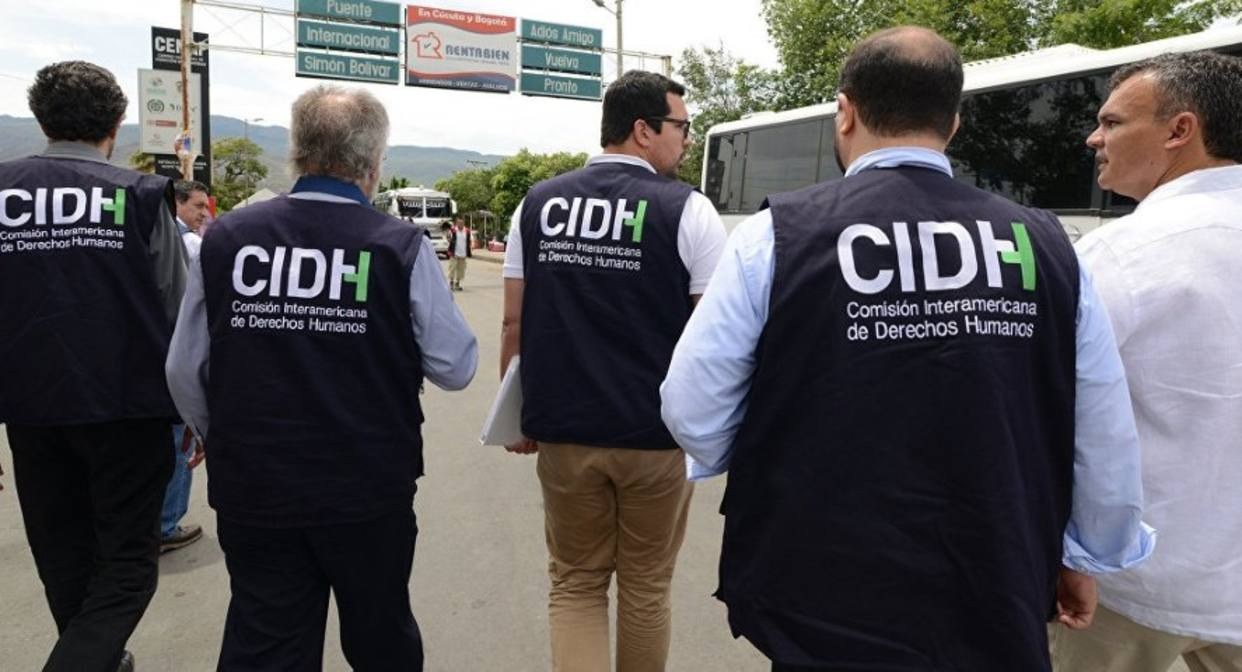
\includegraphics[width=300px]{213.jpg}%
\newline%
%
La Comisión Interamericana de Derechos Humanos (CIDH) exigió este jueves una investigación imparcial para determinar lo sucedido en la muerte de Fernando Albán, concejal del municipio Libertador.%
\newline%
%
La CIDH condenó la muerte de Albán mientras se encontraba bajo custodia en la sede del Servicio~Bolivariano de Inteligencia Nacional (Sebin), ubicado en Plaza Venezuela.%
\newline%
%
"CIDH condena muerte de concejal Fernando Albán mientras estaba bajo custodia del Servicio Bolivariano de Inteligencia Nacional (Sebin) en Venezuela y exige una investigación pronta, exhaustiva e imparcial para determinar lo ocurrido y aplicar las sanciones que correspondan" dijo la organización en su Twitter.%
\newline%
%
El 5 de octubre el concejal por Primero Justicia fue detenido por funcionarios del Sebin en el Aeropuerto Internacional Simón Bolívar, ubicado en Maiquetía, estado Vargas,~ por estar presuntamente vinculado con el "atentado" en contra del presidente Nicolás Maduro.%
\newline%
%
Tarek William Saab, fiscal general designado por la asamblea nacional constituyente, informó la muerte de Albán en la sede del Sebin. Indicó que el dirigente se lanzó del piso 10 del edificio.%
\newline%
%
\end{document}